\documentclass{article}
\usepackage[utf8]{inputenc}
\usepackage{amsmath}
\usepackage{amssymb}
\usepackage{graphicx}



\begin{document}
\section*{Economical Singular-Value Decomposition}
Given a matrix $\mathbf{A}\in \mathbb{R}^{m,n}$, $m, n \in \mathbb{N}$, $\mathbf{A} \neq \mathbf{O}$, we write 
\begin{equation*}
    \mathbf{A} = \mathbf{U}\mathbf{\Sigma}\mathbf{V}^{\mathsf{T}}
\end{equation*}
for its \textbf{economical (thin) SVD}

\subsection*{3-14.a}
We are tasked with filling in the correct matrix sizes.

\begin{figure}[!hbt]
    \centering
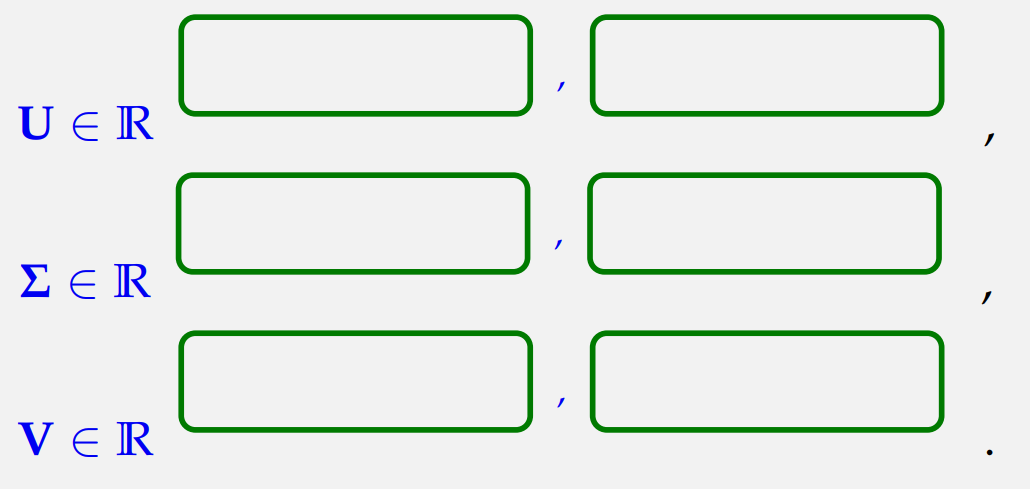
\includegraphics[width=0.7\linewidth]{ThinSVDMatrixSizes.png}
\end{figure}
\noindent We know that $\mathbf{\Sigma}$ will be square and contain for each non-zero eigenvalue of $\mathbf{A}^{\mathsf{T}}\mathbf{A}$ and $\mathbf{A}\mathbf{A}^{\mathsf{T}}$ an non-zero singular value of $\mathbf{A}$ which is the square root of one of these eigenvalues. Hence the matrix $\mathbf{\Sigma}$ will always be square. We have For $\mathbf{A} \in \mathbb{R}^{m,n}$ that $\mathbf{A}^{\mathsf{T}}\mathbf{A} \in \mathbb{R}^{n,n}$ and $\mathbf{A}\mathbf{A}^{\mathsf{T}} \in \mathbb{R}^{m,m}$. We then look at Lemma 3.4.1.13. which states that the number of (not necessarily non-zero) are given by $\text{min}\left\{m,n\right\}$ of which $r = \text{rank}\left(\mathbf{A}\right)$ is the number of non-zero singular values. Hence we have $\mathbf{\Sigma}\in \mathbb{R}^{\text{min}\left\{m,n\right\}}$, however we would optimally only store $r$ many, as the others are zero. Now we have two cases $m \geq n$ and $m < n$. For $m \geq n$ we can see that $\mathbf{\Sigma}\in \mathbb{R}^{n,n}$ and we hence (regard that the matrix multiplication of the SVD must give us a matrix of dimensions $m \times n$ and must be compatible) get $\mathbf{U}\in \mathbb{R}^{m,n}$ and $\mathbf{V}\in \mathbb{R}^{n,n}$. In the other case we get $\mathbf{U}\in \mathbb{R}^{m,m}$ and $\mathbf{V}^{\mathsf{T}}\in \mathbb{R}^{m,n} \implies \mathbf{V}\in \mathbb{R}^{n,m}$

\begin{align*}
    m \geq n&: \: \mathbf{A} = \mathbf{U}\mathbf{\Sigma}\mathbf{U}^{\mathsf{T}}\,,\: \mathbf{U}\in \mathbb{R}^{m,n}\,,\:\mathbf{\Sigma}\in\mathbb{R}^{n,n}\,,\: \mathbf{V}\in\mathbb{R}^{n,n} \\
     m < n&: \:
    \mathbf{A} = \mathbf{U}\mathbf{\Sigma}\mathbf{U}^{\mathsf{T}}\,,\: \mathbf{U}\in \mathbb{R}^{m,m}\,,\:\mathbf{\Sigma}\in\mathbb{R}^{m,m}\,,\: \mathbf{V}\in\mathbb{R}^{n,m}
\end{align*}
We can compress this into 
\begin{equation*}
    \mathbf{A} = \mathbf{U}\mathbf{\Sigma}\mathbf{U}^{\mathsf{T}}\,,\: \mathbf{U}\in \mathbb{R}^{m,\text{min}\left\{m,n\right\}}\,,\:\mathbf{\Sigma}\in\mathbb{R}^{\text{min}\left\{m,n\right\},\text{min}\left\{m,n\right\}}\,,\: \mathbf{V}\in\mathbb{R}^{n,\text{min}\left\{m,n\right\}}
\end{equation*}

\pagebreak

\subsection*{3-14.b}
We are tasked sith deciding whether the following statement are true for \textbf{every} $\mathbf{A}\in \mathbb{R}^{m,n} \setminus \left\{\mathbf{O}\right\}$, $m,n\in \mathbb{N}$.
\paragraph{1. The matrix $\mathbf{U}$ is an orthogonal matrix:} We have seen above that both $\mathbf{U}$ and $\mathbf{V}$ do not have to be square matrices in the economical SVD, hence only in the full SVD we get that both $\mathbf{U}$ and $\mathbf{V}$ are orthogonal. Hence this statement is \textbf{FALSE}.
\paragraph{2. The set of all columns of $\mathbf{U}$ is an orthonormal basis of $\mathcal{R}\left(\mathbf{A}\right)$:} The column of $\mathbf{U}$ and $\mathbf{V}$ will be orthonormal, however they may not be square and would thus not represent a basis of $\mathcal{R}\left(\mathbf{A}\right)$. For example if $m \geq n$ and $\text{rank}\left(\mathbf{A}\right) < n$, then the columns of $\mathbf{U}$ will span a a space of dimension $n$ as the columns are $n$ orthonormal vectors, because of $\text{rank}\left(\mathbf{A}\right) < n$ we have that $\mathcal{R}\left(\mathbf{A}\right)$ has a smaller dimension. Hence the statement is \textbf{FALSE}.
\paragraph{3. $\mathbf{V}$ has orthogonal rows:} Only the columns of $\mathbf{V}$ have to be orthogonal (due to being orthonormal), this does not make any statement about the rows. Let us consider the case where $m < n$, we then have that $\mathbf{V}\in\mathbb{R}^{n,m}$ which mean that we have $n$ rows of length $m$ where $m < n$, hence these rows cannot be orthogonal to each other as otherwise this would imply that they are linearly independent, which would result in us having found more linearly independent columns than the dimension of the space they span, which is not possible. As a consequence the statement is \textbf{FALSE}.
\paragraph{4. $\mathbf{V}^{\mathsf{T}}\mathbf{V}=\mathbf{I}$:} 
We discussed that the rows of $\mathbf{V}$ must not necessarily be orthonormal, the columns are by definition orthonormal and thus $\mathbf{V}^{\mathsf{T}}$ must have orthonormal rows and thus we have that $\mathbf{V}^{\mathsf{T}}\mathbf{V} = \mathbf{I}$, but it is possible that $\mathbf{V}\mathbf{V}^{\mathsf{T}} \neq \mathbf{I}$. The statement is \textbf{TRUE}.

\paragraph{5. nnz$\left(\Sigma\right):=\#\left\{\left(i,j\right)\::\: \left(\Sigma\right)_{i,j}\neq 0\right\} \leq n$: } We have seen that the matrix $\mathbf{\Sigma}$ contains only non-zero entries on its diagonal and only at most $\text{rank}\left(\mathbf{A}\right)$. We know that because can be at most the number of rows of $\mathbf{A}$ we have $\text{rank}\left(\mathbf{A}\right) \leq m$ and because we have $\mathbf{\Sigma}\in \mathbb{R}^{\text{min}\left\{m,n\right\},\text{min}\left\{m,n\right\}}$ we always have at most $n$ such entries as because if $n <= m$, then there are exactly $n$ diagonal entries, and if $m > n$, then we still have $\text{rank}\left(\mathbf{A}\right) \leq n$, because the column rank and the row rank must match, hence again at most $n$ such entries. The statement is thus \textbf{TRUE}.

\paragraph{6. $\mathbf{U}\mathbf{V}^{\mathsf{T}} = \mathbf{I}$:} These two matrices are not related to each other, hence the statement is \textbf{FALSE}. This can be proven with a counterexample.
\begin{equation*}
    \begin{bmatrix}
    3 & 1 \\
    0 & 4
    \end{bmatrix} = 
    \begin{bmatrix}
        \frac{1}{\sqrt{5}} & -\frac{2}{\sqrt{5}} \\
        \frac{2}{\sqrt{5}} & -\frac{1}{\sqrt{5}}
    \end{bmatrix} 
    \begin{bmatrix}
        3\sqrt{2} & 0 \\
        0 & 2\sqrt{2}
    \end{bmatrix}
    \begin{bmatrix}
        \frac{1}{\sqrt{10}} & -\frac{3}{\sqrt{10}} \\
        \frac{3}{10} & \frac{1}{\sqrt{10}}
    \end{bmatrix}^{\mathsf{T}} \text{ \textbf{but} } \begin{bmatrix}
        \frac{1}{\sqrt{5}} & -\frac{2}{\sqrt{5}} \\
        \frac{2}{\sqrt{5}} & -\frac{1}{\sqrt{5}}
    \end{bmatrix}  \begin{bmatrix}
        \frac{1}{\sqrt{10}} & -\frac{3}{\sqrt{10}} \\
        \frac{3}{\sqrt{10}} & \frac{1}{\sqrt{10}}
    \end{bmatrix}^{\mathsf{T}} = \begin{bmatrix}
        -\frac{1}{\sqrt{2}} &  -\frac{1}{\sqrt{2}} \\
         \frac{1}{\sqrt{2}} &  -\frac{1}{\sqrt{2}}
    \end{bmatrix} 
\end{equation*}

\subsection*{3-14.c}
What is the asymptotic computational effor for computing the economical SVD of a dense matrix $\mathbf{A}\in \mathbb{R}^{m,n}$, $m,n \in  \mathbb{N}$?
\begin{equation*}
    \text{cost}\left(\text{economical SVD of 
 $\mathbf{A}\in \mathbb{R}^{m,n}$}\right) = \mathcal{O}\left(\text{min}\left\{m,n\right\}^{2}, \text{max}\left\{m,n\right\}\right)
\end{equation*}
this can be derived from the implementation of the Eigen \verb|JacobiSVD| which states that the complexity is $\mathcal{O}\left(n^{2}p\right)$, where $n$ is the smaller dimension and $p$ is the greater dimension.

\end{document}
